
\subsection{Experimental Result of ASR Expansion on Mechanical Properties of Concrete}

% [Swamy & Al-Asali, 1988]
In first test study, Swamy and Asali\cite{Swamy} observed ASR-affected concrete in views of compressive strength, using 3 types Mixes (Control, 41/2\% opal, 15\% fused silica) for 1 year, in a cubic shape of size 100x100x100mm. The expansion is measured one-dimensionally.

The results found are in Figure \ref{Swamy1} as follow [Swamy \& Al-Asali, 1988] .

\begin{figure}[h!]
  \centering
  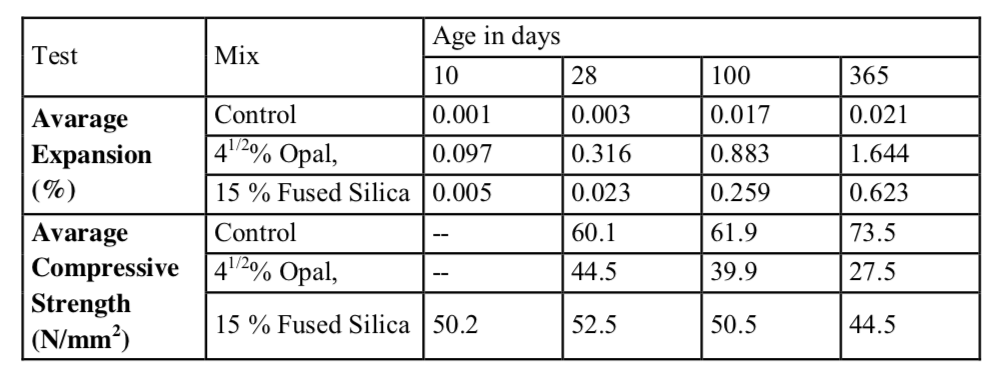
\includegraphics[width=0.8\linewidth]{Reference/temp3.png}
  \caption{Effects of ASR expansion on compressive strength of concrete [Swamy \& Al-Asali, 1988].}
  \label{Swamy1}
\end{figure}


The compressive strength of opal concrete was 54\% less than that the control concrete for 28 days, then reached to 63\% at 1 year compared with the strength of control concrete. The loss in strength of fused silica concrete was nearly 26\% at 28 days and 39\% at 1 year as comparing it with that of control concrete [Swamy \& Al-Asali, 1988].

In Figure \ref{Swamy, Al-Asali, 1988 2}, the loss in compressive strength of control concrete and ASR-affected concrete at different rates of expansion was shown, where drop of compressive strength of ASR-affected concretes becomes more clear with expansion [Swamy \& Al-Asali, 1988].

\begin{figure}[h!]
\centering
%*******
\begin{subfigure}{.8\textwidth}
  \centering
  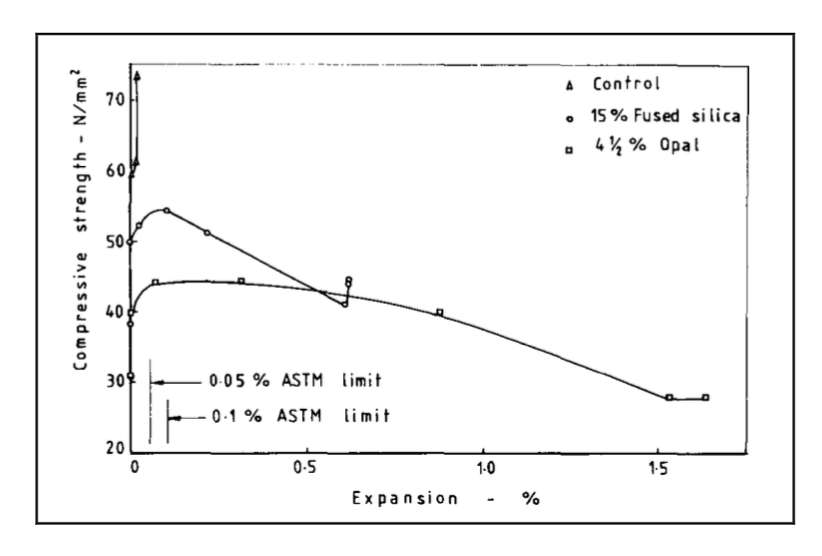
\includegraphics[width=1.0\linewidth]{Reference/temp5.png}
\end{subfigure}
%*******
\begin{subfigure}{.8\textwidth}
  \centering
  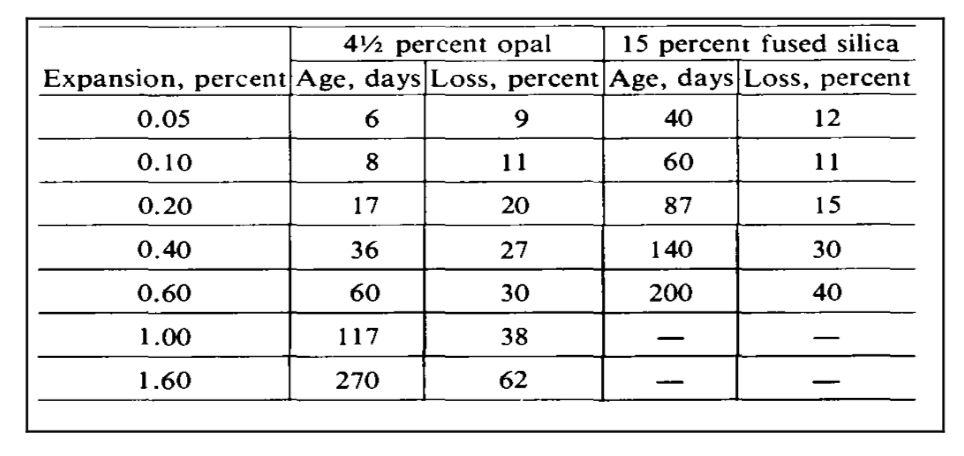
\includegraphics[width=1.0\linewidth]{Reference/temp6.png}
\end{subfigure}
%*******
\caption{Loss of compressive strength of ASR-affected concrete with time [Swamy \& Al-Asali, 1988]}
\label{Swamy, Al-Asali, 1988 2}
\end{figure}

\clearpage
%[Ahmed et al., 2003]
T. Ahmed et al.\cite{Ahmed} used Thames Valley sand (in Mix A), fused silica (in Mix B) and slowly reactive aggregate (in Mix C) to investigate the effect of ASR expansion on compressive strength of concrete, using specimens in size of 100x100x100 mm[BSEN 1290-3, 2000], cast and cured with respect to BS 1881 Part 122 [BS, 1881].

In this experiment, the cube specimens were cured for 28 days in water at 20$^\circ$C nd then the temperature was increased to 38$^\circ$C to accelerate alkali-silica reaction. Then specimens were stored at water tank until 12 months passed [Ahmed et al., 2003]. After 28-days curing at 20$^\circ$C and storage at 38$^\circ$C for 12 months, the expansion ratios and compressive strength are given in Figure \ref{Ahmed et al., 2003 1} [Ahmed et al., 2003].

% TODO: Remake Figure

\begin{figure}[h!]
  \centering
  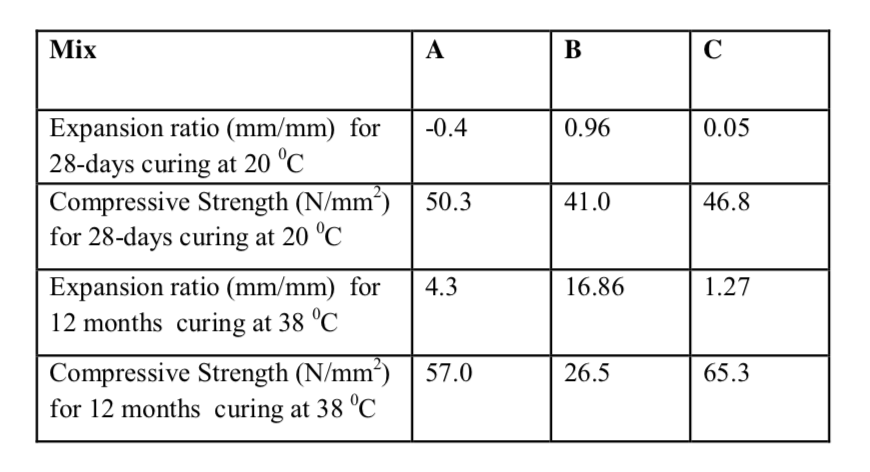
\includegraphics[width=0.8\linewidth]{Reference/temp1.png}
  \caption{Effect of ASR expansion on compressive strength of concrete [Ahmed et al., 2003].}
  \label{Ahmed et al., 2003 1}
\end{figure}

As seen in Figure \ref{Ahmed et al., 2003 1}, the results reveal that compressive strength of Mix A is nearly 7.5\% higher than Mix C's (control mix) at 28 days due to no expansion in Mix A, while compressive strength of Mix A is nearly 12.7\% less than Mix C's (control mix) at 12 months due to its greater expansion compared with expansion of Mix C. As for Mix B, which is with fused silica, the greatest expansion in the three mixes is achieved and compressive strength dropped nearly 12.4\% for 28 days with compared to Mix C. After stored at hot water (38$^\circ$C) for 12 months, the drop in strength of Mix B reached to nearly 59.4\% [Ahmed et al., 2003].

%TODO: CHECK This
%As an another views, Cope and Slade observed an compressive strength increase in same mix (Mix A) and claimed that the curing of concrete including slowly reactive aggregate at high temperature doesn't affect overly on compressive strength of concrete at an early age or even after plenty time passes so compressive strength of Mix A can increase at 38$^\circ$C at this time [Cope & Slade, 1992].

Figure 3.1 reveals that a greater decrease in compressive strength was observed in Mix B compared with Mix A at any expansion percent due to different reaction rates for fused silia and Thames Vally sand permitting the hydration of cement to increase the compressive strength of concrete [Ahmed et al., 2003].

\begin{figure}[h!]
  \centering
  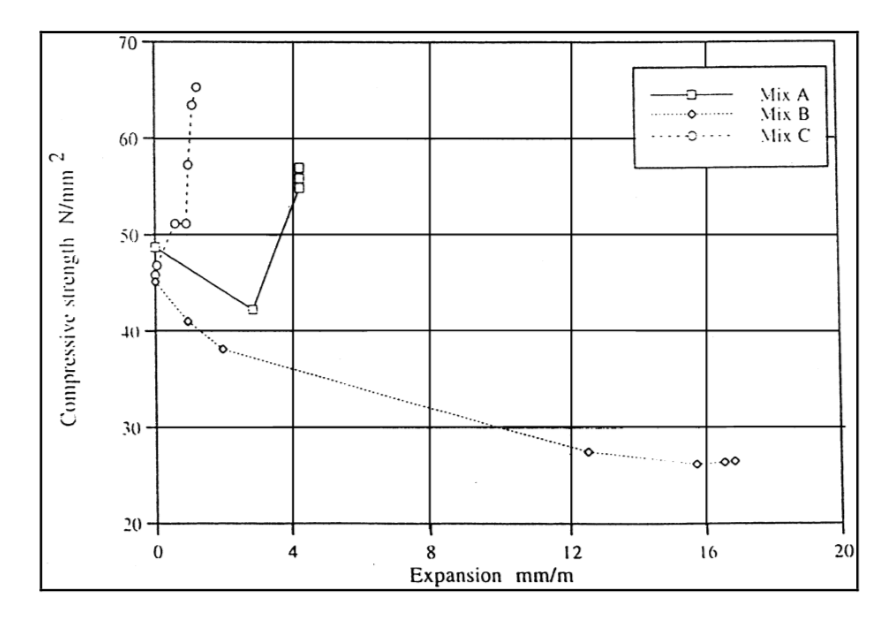
\includegraphics[width=0.8\linewidth]{Reference/temp2.png}
  \caption{Change in compressive strength of ASR-affected concrete vs. time [Ahmed et al., 2003].}
  \label{Ahmed et al., 2003 2}
\end{figure}

\clearpage
% GIANNINI(2012)

Giannini\cite{GIANNINI} carried out mechanical properties test on expanded specimens damaged by ASR and DEF expansion. Two sets of 4 x 8 in. (100 x 200 mm) cylinders were produced for the purpose of further evaluating the effects of ASR and DEF on the mechanical properties of concrete. This study expands on and complements the mechanical tests conducted on the core samples extracted from the exposure site specimens. Two reactive aggregates, Jobe (F1) sand and Placitas (C10) gravel were used, bringing the total number of reactive aggregates investigated in the overall project to four. A non-linear resonant frequency test method was also employed for selected test specimens. In this study, the cylinders are intended to represent a laboratory analog for core samples extracted from a field structure.

Here the experiment results for ASR expansion are presented. Figure \ref{Giannini, 2012} shows the compressive strength results for the Jobe (F1) andPlacitas (C10) cylinders, respectively. Each data represents the average of three cylinders.

For the Jobe (F1) cylinders, decreases of 15\% were measured. For the Placitas (C10) cylinders, an increase of 17\% was measured for the ASR cylinders. The Placitas (C10) ASR cylinders expanded much more slowly than all other specimens in this study, and therefore were able to gain strength (possibly due to continued hydration of cement) more quickly than ASR could degrade it. However, the strength at 0.177\% expansion (approximately 8 months of age) was almost 18\% lower than that of the non-reactive control specimens at one year, so ASR did still have a negative impact on strength.

\begin{figure}[h!]
  \centering
  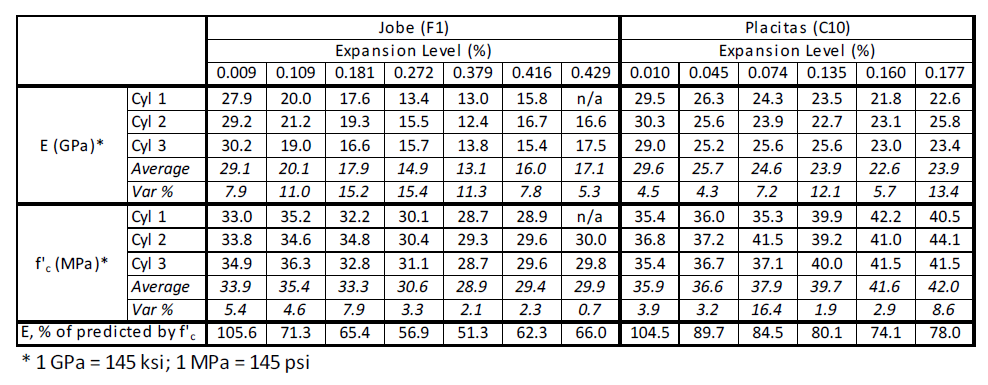
\includegraphics[width=0.8\linewidth]{Reference/GIANNINIASR.png}
  \caption{Elastic modulus and compressive strength results for ASR cylinders[Giannini, 2012]}
  \label{Giannini, 2012}
\end{figure}

\clearpage
%ALKANA(2013)

In study done by ALKANA (2014)\cite{ALKANA}, the effect of ASR expansion on mechanical properties of concrete and the effect of specimen types on ASR expansion were investigated. Mechanical tests were performed on both the specimens exceeding expansion from ASR of 0.04 percent and ones exceeding that of 0.10 percent.

In this part, the results for G-A concrete with greater than expansion of 0.04 percent, G-B concrete with greater than that of 0.10 percent, and G-C concrete (control concrete) were given with graphs and tables in the following parts. While ASR-affected concrete (G-A, G-B) were started to be stored at 60$^\circ$C and 100\% RH, G-B concrete was compulsorily exposed to NaOH solution in recent weeks in order to provide expansion percentage of G-B concrete to exceed the limit of 0.10 percent. G-C concrete, on the other hand, was cured in water at 20$^\circ$C and used as control concrete. As known, the formed ASR gel absorbs water, expands, and causes internal pressure that causes cracking, which then continues and leads to expansion in concrete structure.



The ASR effect on compressive strength was examined by using cubic specimens, 150x150 mm in size, and cylindrical specimens, 100x200 mm in size. While the mix design of all specimens was prepared according to regulations as described by RILEM TC 219-ACS, compressive test for all specimens were carried out in accordance with the provisions in TS EN 12390-3. Limestone, non-reactive aggregate, and natural river sand, moderately reactive aggregate, were used as coarse and fine aggregates, respectively.

The expansion results in compressive strength for all specimens are given Figure \ref{ALKANA1}, Figure \ref{ALKANA2} and Figure \ref{ALKANA3}.

\begin{figure}[h!]
  \centering
  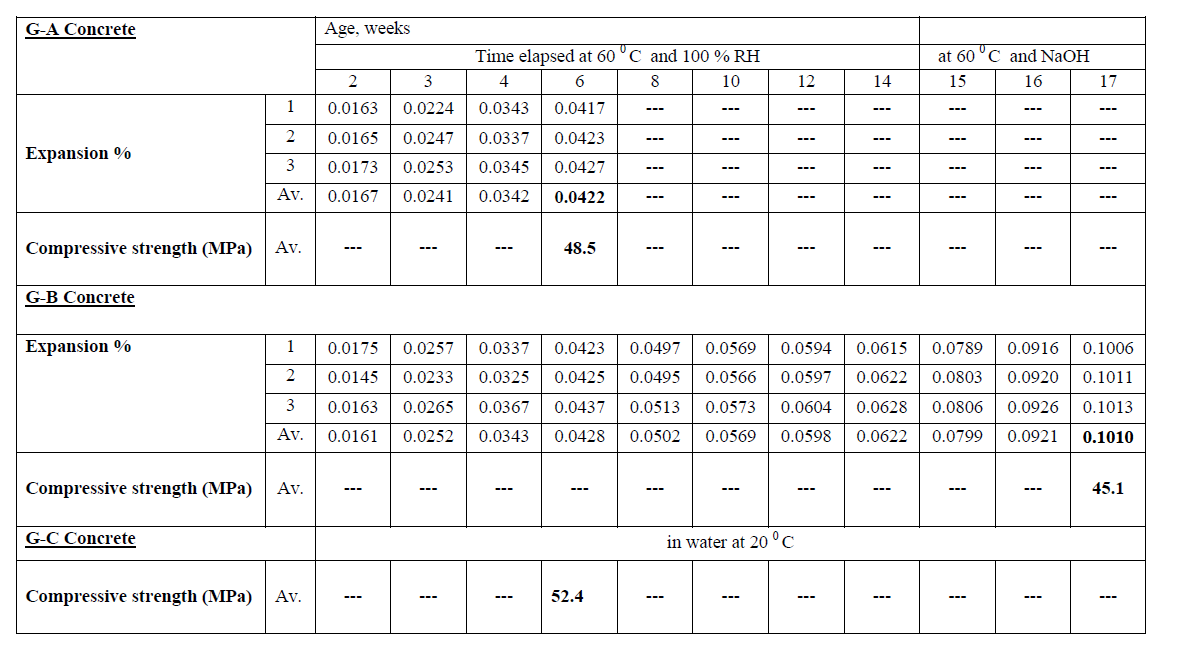
\includegraphics[width=1.0\linewidth]{Reference/ALKANASR1.png}
  \caption{Expansion and compressive strength of all concretes for cube specimens[ALKANA, 2012]}
  \label{ALKANA1}
\end{figure}

\begin{figure}[h!]
  \centering
  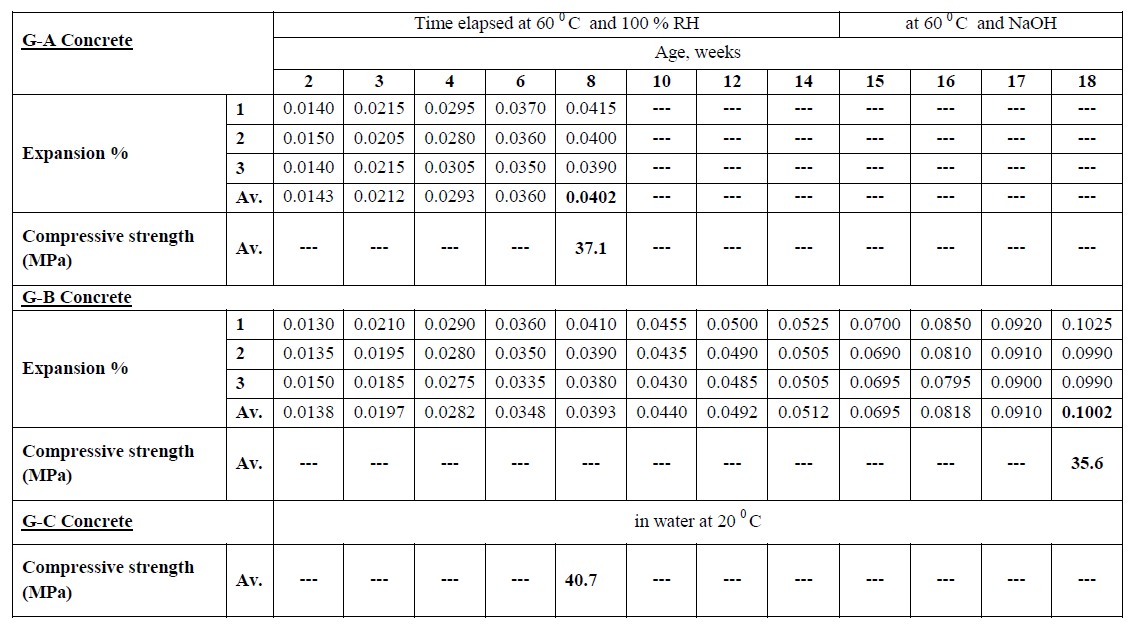
\includegraphics[width=1.0\linewidth]{Reference/ALKANASR2.png}
  \caption{Expansion and compressive strength of all concretes for cylindrical specimens[ALKANA, 2012]}
  \label{ALKANA2}
\end{figure}

\begin{figure}[h!]
  \centering
  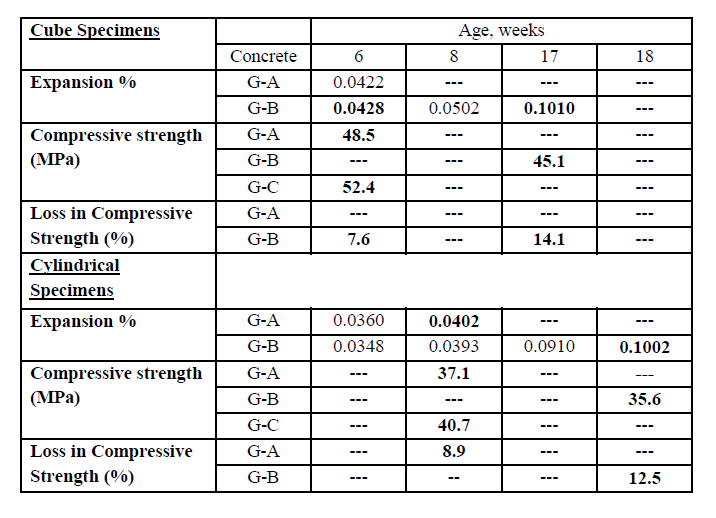
\includegraphics[width=1.0\linewidth]{Reference/ALKANASR3.png}
  \caption{Loss in compressive strength of ASR-affected concrete comparing with control concrete [ALKANA, 2012]}
  \label{ALKANA3}
\end{figure}

\clearpage
\subsection{Summary of Experimental Result of ASR Expansion on Mechanical Properties of Concrete}

\begin{figure}[h!]
  \centering
  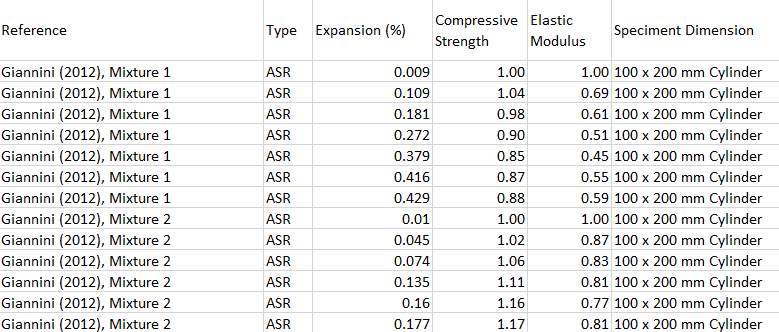
\includegraphics[width=1.0\linewidth]{Reference/GIANNINIASRdata.png}
\end{figure}

\begin{figure}[h!]
  \centering
  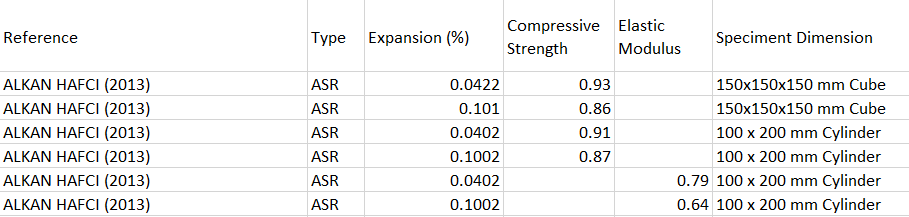
\includegraphics[width=1.0\linewidth]{Reference/ALKANASRdata.png}
\end{figure}

\begin{figure}[h!]
  \centering
  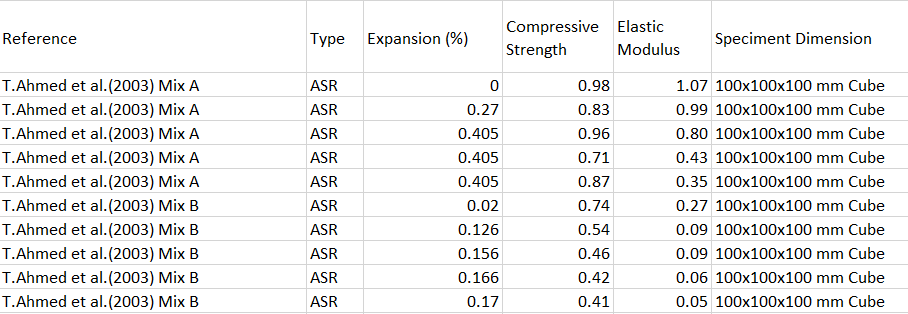
\includegraphics[width=1.0\linewidth]{Reference/AhmedASRdata.png}
\end{figure}

\begin{figure}[h!]
  \centering
  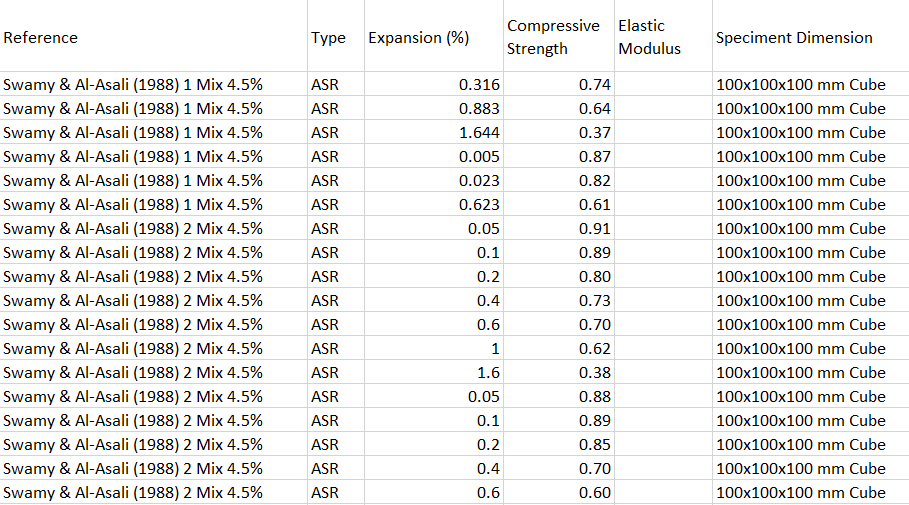
\includegraphics[width=1.0\linewidth]{Reference/SwamyASRdata_1.png}
\end{figure}

\begin{figure}[h!]
  \centering
  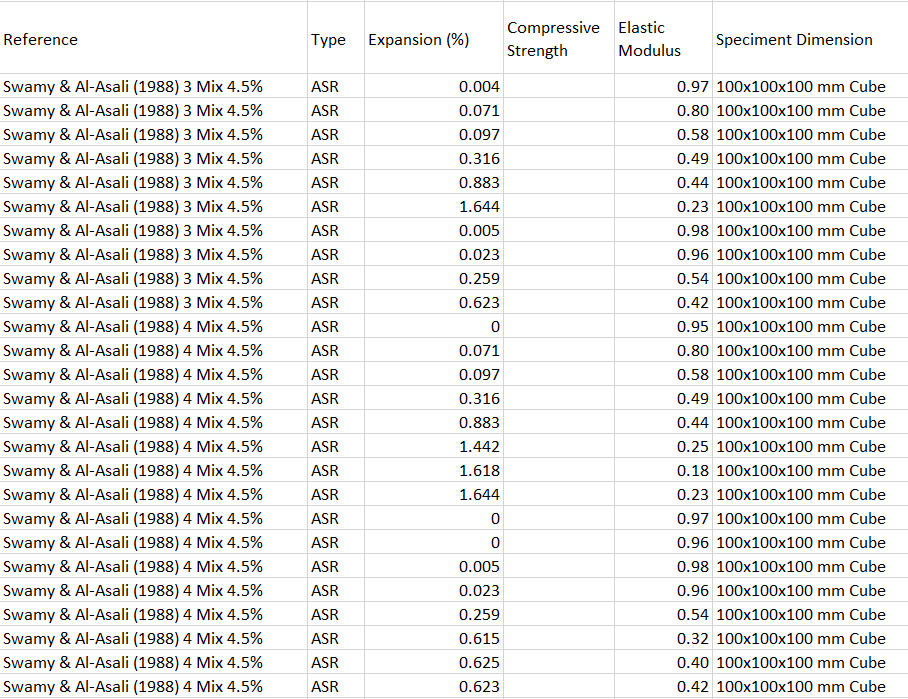
\includegraphics[width=1.0\linewidth]{Reference/SwamyASRdata_2.png}
\end{figure}


% \begin{table}[ht!]
% \centering
% \begin{tabular}{  ||p{2.2cm}|p{2.2cm}|p{2.2cm}|p{2.2cm}|p{2.2cm}|p{2.2cm}|| }
% \hline
%  Reference & Type & Expansion (\%) & Compressive Strength Remained & Specimen Dimension \\
%   \hline
%
%
%
%   \hline
%   \end{tabular}
% \caption{Expansion in Each Step for A30 Case 3}
% \label{table:A30X0C_3_EXP}
% \end{table}
